\documentclass{beamer}
\usepackage{graphicx}
\usepackage{geometry}
\usepackage[ngerman]{babel}
\usetheme{Warsaw}

\usepackage{xcolor}
\usepackage{listings}
\lstset{
backgroundcolor=\color{white},
basicstyle=\footnotesize,
breakatwhitespace=false,
breaklines=true,
captionpos=b,
commentstyle=\color{gray}\textit,
frame=tb,
keepspaces=true,
keywordstyle=\color{blue}\bfseries,
language=erlang,
numberstyle=\tiny\color{gray},
rulecolor=\color{black},
showspaces=false,
showstringspaces=false,
showtabs=false,
stepnumber=1,
stringstyle=\color{violet},
tabsize=2,
title=\lstname,
columns=fixed
}

\makeatletter
\newcommand\titlegraphicii[1]{\def\inserttitlegraphicii{#1}}
\titlegraphicii{}
\setbeamertemplate{title page}
{
\vbox{}
{\usebeamercolor[fg]{titlegraphic}\inserttitlegraphic\hfill\inserttitlegraphicii\par}
\begin{centering}
    \begin{beamercolorbox}[sep=8pt,center]{institute}
        \usebeamerfont{institute}\insertinstitute
    \end{beamercolorbox}
    \begin{beamercolorbox}[sep=8pt,center]{title}
        \usebeamerfont{title}\inserttitle\par%
        \ifx\insertsubtitle\@empty%
        \else%
        \vskip0.25em%
        {\usebeamerfont{subtitle}\usebeamercolor[fg]{subtitle}\insertsubtitle\par}%
        \fi
        %
    \end{beamercolorbox}%
    \vskip1em\par
    \begin{beamercolorbox}[sep=8pt,center]{date}
        \usebeamerfont{date}\insertdate
    \end{beamercolorbox}%\vskip0.5em
    \begin{beamercolorbox}[sep=8pt,center]{author}
        \usebeamerfont{author}\insertauthor
    \end{beamercolorbox}
\end{centering}
%\vfill
}
\makeatother
\author{Adrian Helberg}
\title{Referat - Pr\"asentation}
\subtitle{Aufgabe 3 - Flu\ss{}probleme}
\date{\today}
\titlegraphicii{
\includegraphics[height=1.8cm]{../haw_logo.png}}

\begin{document}

    \begin{frame}[plain]
        \maketitle
        \small
        \\~\\~\\~\\
        \resizebox{\linewidth}{!}{
        \begin{tabular}{l r}
            \textit{Pr\"ufer}: & Prof. Dr. C. Klauck\\
            \textit{Vorlesung}: & Graphentheoretische Konzepte und Algorithmen
        \end{tabular}}
    \end{frame}

    \begin{frame}{Inhalt}
        \tableofcontents
    \end{frame}

    \section{Einleitung}
    \begin{frame}{Einleitung - Selbstorganisation}
        \begin{center}
            \begin{tabular}{l | r}
                Arbeitspaket & Zeitabsch\"atzung (in Stunden) \\
                \hline
                Recherche & 2-3\\
                Algorithmen verstehen & 4-5\\
                Entwurf & 16\\
                Implementierung & 16
            \end{tabular}
        \end{center}
    \end{frame}

    \section{Kontext}
    \begin{frame}{Kontext - Aufgabenstellung}
        \begin{block}{Aufgabenstellung}
            \begin{itemize}
                \item Der Algorithmus von \textbf{Ford und Fulkerson} \footnote{" `Ford-Fulkerson"', 1956, L.R.Ford \& D.R.Fulkerson}
                \item Der Algorithmus von \textbf{Edmonds und Karp} \footnote{"`Edmonds-Karp"', 1970, Yefim Dinitz, 1972, J.Edmonds \& R.Karp}
                \item Algorithmen \textit{ohne} Residualnetzwerk
                \item Nachvollziehbare Ergebnisse (Erstellen von Log-Dateien, Generierung von SVG-Dateien, etc.)
                \item \textit{printGFF}
                \item Nachweise einer erwarteten Komplexit\"at
                \item Laufzeitmessungen
            \end{itemize}
        \end{block}
    \end{frame}

    \begin{frame}{Kontext - Algorithmen}
        \begin{center}
            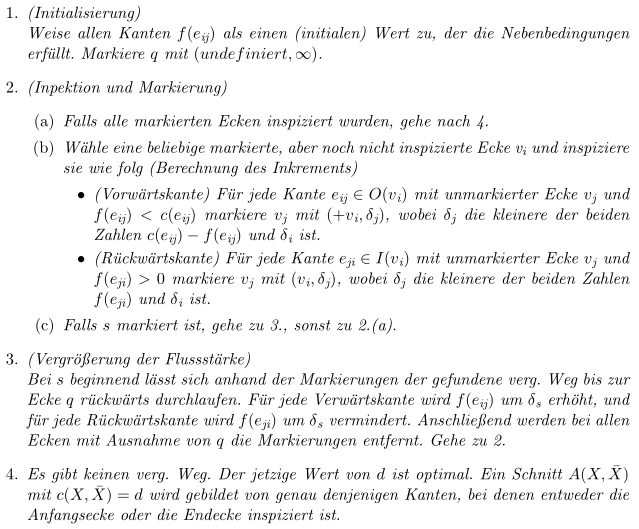
\includegraphics[height=6.8cm]{../algorithmus.PNG}
        \end{center}
    \end{frame}

    \begin{frame}{Kontext - Algorithmen}
        \begin{block}{Besonderheiten}
            \begin{itemize}
                \item \textbf{Ford-Fulkerson} und \textbf{Edmonds-Karp} unterscheiden sich nur in der Suchreihenfolge nach einem vergr. Weg.
                \item \textbf{Edmonds-Karp} verwendet hierzu eine \textit{Queue}
                \item Durch den spezifizierten R\"uckgabewert\\
                $[($\textit{Liste der im letzten Lauf inspizierten Knoten}$)]$\\
                kann Schritt 4. der Algorithmen vernachl\"assigt werden
            \end{itemize}
        \end{block}
    \end{frame}

    \begin{frame}{Kontext - Komplexit\"at}
        \begin{block}{aus 1. \textit{(Initialisierung)}}
            \begin{itemize}
                \item Setzen von Werten: \textit{O(1)}
                \item Iterieren von Kanten: \textit{O(N)}
            \end{itemize}
        \end{block}
        \begin{block}{aus 2. \textit{(Inspektion und Markierung)}}
            \begin{itemize}
                \item Markierung/Inspektion pr\"ufen: \textit{O(1)}
                \item Iterieren von Knoten: \textit{O(N)}
            \end{itemize}
        \end{block}
    \end{frame}

    \begin{frame}{Kontext - Komplexit\"at}
        \begin{block}{aus 2. (b)}
            \begin{itemize}
                \item W\"ahlen einer beliebigen Ecke: \textit{O(N)}
                \item W\"ahlen der n\"achsten Ecke aus der Queue: \textit{O(1)}
                \item Inzidente Kanten abfragen: \textit{O(1)}
            \end{itemize}
        \end{block}

        \begin{block}{Erwartete Komplexit\"at}
            \begin{itemize}
                \item \textit{O(Anzahl Kanten x Maximale Anzahl an vergr. Wegen)}
                \item \textit{O(Anzahl Knoten x Anzahl Kanten x Anzahl Kanten)}
            \end{itemize}
        \end{block}
    \end{frame}

    \section{Entwurf}
    \begin{frame}{Entwurf}
        \begin{block}{Definition}
            \begin{itemize}
                \item Alleinige Vorlage zu einer m\"oglichen Implementierung unabh\"agig zur Programmiersprache
                \item M\"ogliche Probleme schnell erkennen, um Aufwand zu minimieren
                \item Grundlegendes f\"ur effiziente Implementierungen und damit gute Softwarel\"osungen schaffen
            \end{itemize}
        \end{block}
    \end{frame}

    \begin{frame}{Entwurf - Algorithmen}
        \begin{block}{Wirkungsprinzip}
            \begin{center}
                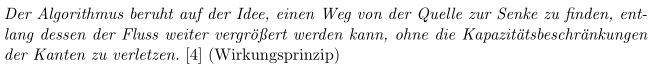
\includegraphics[width=10.8cm]{../wirkungsprinzip.PNG}
            \end{center}
        \end{block}

        \begin{block}{Informationen an Ecken und Kanten}
            \begin{itemize}
                \item Ecken: $(+/-$,Vorg\"anger,$\delta)$
                \item Kanten: Fluss, Kapazit\"at
            \end{itemize}
        \end{block}
    \end{frame}

    \begin{frame}{Entwurf - Datenstrukturen}
        \begin{block}{Allgemein}
            Effiziente Organisation von Daten mit Listen und Tupeln
        \end{block}
        \begin{block}{aus 1. \textit{(Initialisierung)}}
            \begin{itemize}
                \item Setzen eines initialen Flusses durch rekursives Durchlaufen aller Kanten
            \end{itemize}
        \end{block}
        \begin{block}{aus 2. \textit{(Inspektion und Markierung)}}
            \begin{itemize}
                \item Knoten werden durch die Informationen "`Vorzeichen"', "`Vorg\"anger"' und "`Delta"' markiert
                \item Knoten werden inspiziert
            \end{itemize}
        \end{block}
    \end{frame}

    \begin{frame}{Entwurf - Datenstrukturen}
        \begin{block}{aus 2. (b)}
            \begin{itemize}
                \item Ermitteln einer beliebigen Ecke / Holen einer Ecke aus der Queue
                \item Holen der Inzidenten Kanten der Ecke
            \end{itemize}
        \end{block}

        \begin{block}{aus 2. \textit{(Vergr\"o\ss{}erung der Flussst\"arke)}}
            \begin{itemize}
                \item Knoten der L\"aufe von Vergr\"o\ss{}erung sind zu halten (R\"uckgabewert)
            \end{itemize}
        \end{block}
    \end{frame}

    \begin{frame}{Entwurf - Programmfluss}
        \begin{center}
            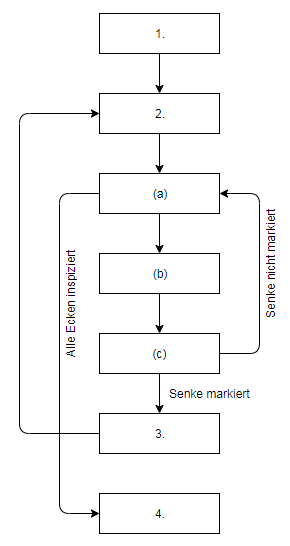
\includegraphics[width=3.6cm]{../fordfulkerson.PNG}
        \end{center}
    \end{frame}

    \section{Laufzeitmessung}
    \begin{frame}{Laufzeitmessung}
        \begin{block}{Idee}
            \begin{itemize}
                \item[I.] Erfassen der Laufzeitkomplexit\"at durch skalierende Eingebedaten
                \item[II.] Vergleich beiden Algorithmen
                \item[III.] Herausarbeiten der Unterschiede beider Algorithmen
            \end{itemize}
        \end{block}

        \begin{block}{Idee}
            \begin{itemize}
                \item Nutzen von \textbf{gengraph} zur Erstellung randomisierter Graphen f\"ur Laufzeitexperimente
            \end{itemize}
        \end{block}
    \end{frame}

    \begin{frame}{Laufzeitmessung - Versuchsaufbau}
        \begin{block}{zu I.}
            \begin{center}
                \begin{tabular}{c|c|c}
                    \textbf{Edmonds-Karp} & \textbf{Ford-Fulkerson} & Anzahl Ecken (Kanten)\\
                    \hline
                    & & 10 (45)\\
                    & & 20 (190)\\
                    & & 30 (434)\\
                    & & 40 (780)\\
                    & & 50 (1225)\\
                    & & 60 (1770)\\
                    & & 70 (2415)\\
                    & & 80 (3160)\\
                    & & 90 (4005)\\
                    & & 100 (4950)\\
                \end{tabular}
            \end{center}
        \end{block}
    \end{frame}

    \begin{frame}{Laufzeitmessung - Versuchsdurchf\"uhrung}
        \begin{block}{zu I.}
            \begin{center}
                \begin{tabular}{c|c|c}
                    \textbf{Edmonds-Karp} & \textbf{Ford-Fulkerson} & Anzahl Ecken (Kanten)\\
                    \hline
                    5 & 7 & 10 (45)\\
                    22 & 25 & 20 (190)\\
                    79 & 93 & 30 (434)\\
                    217 & 232 & 40 (780)\\
                    443 & 503 & 50 (1225)\\
                    886 & 1001 & 60 (1770)\\
                    1662 & 1896 & 70 (2415)\\
                    2729 & 3072 & 80 (3160)\\
                    5003 & 5144 & 90 (4005)\\
                    8111 & 8785 & 100 (4950)\\
                \end{tabular}
            \end{center}
        \end{block}
    \end{frame}

    \begin{frame}{Laufzeitmessung - Versuchsdurchf\"uhrung}
        \begin{block}{zu II.}
            \begin{center}
                \begin{tabular}{c|c|c}
                    \textbf{Edmonds-Karp} & \textbf{Ford-Fulkerson} & $\delta$\\
                    \hline
                    5 & 7 &\\
                    22 & 25 &\\
                    79 & 93 &\\
                    217 & 232 &\\
                    443 & 503 &\\
                    886 & 1001 &\\
                    1662 & 1896 &\\
                    2729 & 3072 &\\
                    5003 & 5144 &\\
                    8111 & 8785 &\\
                \end{tabular}
            \end{center}
        \end{block}
    \end{frame}

    \begin{frame}{Laufzeitmessung - Versuchsdurchf\"uhrung}
        \begin{block}{zu II.}
            \begin{center}
                \begin{tabular}{c|c|c}
                    \textbf{Edmonds-Karp} & \textbf{Ford-Fulkerson} & $\delta$\\
                    \hline
                    5 & 7 & 2\\
                    22 & 25 & 3\\
                    79 & 93 & 14\\
                    217 & 232 & 15\\
                    443 & 503 & 60\\
                    886 & 1001 & 115\\
                    1662 & 1896 & 234\\
                    2729 & 3072 & 343\\
                    5003 & 5144 & 141\\
                    8111 & 8785 & 674\\
                \end{tabular}
            \end{center}
        \end{block}
    \end{frame}

    \begin{frame}{Laufzeitmessung - Versuchsauswertung}
        \begin{block}{zu III.}
            \begin{center}
                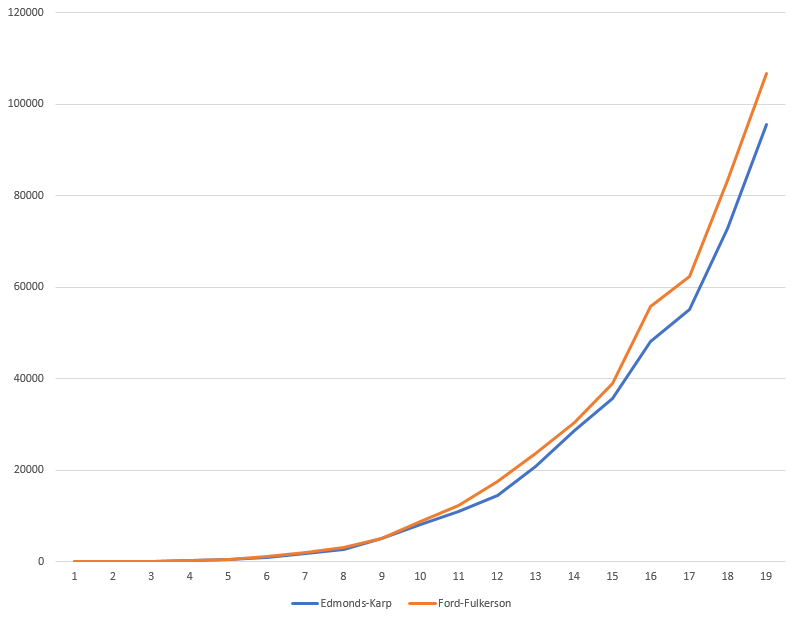
\includegraphics[width=7.8cm]{../auswertung.PNG}
            \end{center}
        \end{block}
    \end{frame}

    \section{Fazit}
    \begin{frame}{Fazit}

    \end{frame}

    \begin{frame}{Ende}
        \begin{center}
            Danke f\"ur Ihre Aufmerksamkeit!
        \end{center}
    \end{frame}

    \begin{frame}{Quellen}
        \begin{center}
            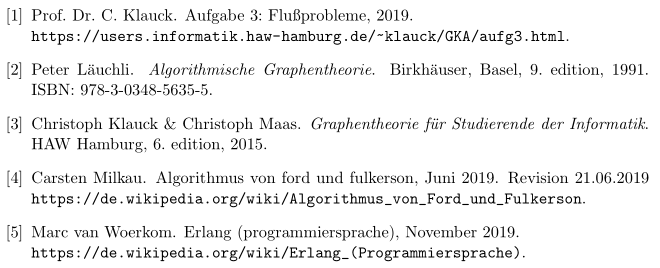
\includegraphics[height=4.4cm]{../quellen.PNG}
        \end{center}
    \end{frame}

\end{document}